\section{From Estimation to Inference}

\begin{frame}{Where We Left Off}
	\begin{itemize}
		\item Fitted the simple linear regression model $\hat y = \hat\beta_0+\hat\beta_1 x$ by least squares
		\item Estimated $\hat\beta_1 = S_{xy}/S_{xx}$ and $\hat\beta_0 = \bar y-\hat\beta_1\bar x$
		\item Estimated $\hat\sigma^2 = MS_E = \frac{SS_E}{n-2} = \frac{\sum_{i=1}^n \hat\varepsilon_i^2}{n-2} = \frac{\sum_{i=1}^n (y_i - \hat y_i)^2}{n-2}$
	\end{itemize}

	\svspace{1em}

	If we drew a different sample, would $\hat\beta_1$ come out the same?
\end{frame}


\section{Sampling Distribution of the OLS Estimators}


\begin{frame}{Sampling Distribution of $\hat\beta_1$}
	\[
		\hat\beta_1 = \frac{S_{xy}}{S_{xx}} = \sum_{i=1}^n c_i Y_i, \qquad c_i=\frac{x_i-\bar x}{S_{xx}}
	\]

	\begin{itemize}
		\item $\hat\beta_1$ is a linear combination of independent normal random variables, therefore, $\hat\beta_1$ is normally distributed
	\end{itemize}

	\pause

	Further,
	\begin{align*}
		E[\hat\beta_1] &= \beta_1 \qquad\text{(unbiased)}\\
		\Var(\hat\beta_1) &= \sigma^2\sum_i c_i^2 = \frac{\sigma^2}{S_{xx}}
	\end{align*}

	\pause
	Therefore:
	\[
		\hat\beta_1 \sim N\!\left(\beta_1,\ \frac{\sigma^2}{S_{xx}}\right)
	\]
\end{frame}


\begin{frame}{Sampling Distribution $\hat\beta_0$}
	Since \(\hat\beta_0 = \bar Y-\hat\beta_1\bar x\) and 
	\begin{align*}
		E[\hat\beta_0] &= \beta_0 \qquad\text{(unbiased)}\\
		\Var(\hat\beta_0) &= \sigma^2\left(\frac1n+\frac{\bar x^2}{S_{xx}}\right)
	\end{align*}

	Therefore:
	
	\[
		\hat\beta_0 \sim N\!\left(\beta_0,\ \sigma^2\left(\frac1n+\frac{\bar x^2}{S_{xx}}\right)\right)
	\]
\end{frame}


\section{Estimating the Error Variance}


\begin{frame}{$\sigma^2$ Is Unknown --- Estimate It from the Residuals}
	\[
		\hat\sigma^2 = MSE = \frac{SSE}{n-2}, \qquad SSE=\sum_{i=1}^n(y_i-\hat y_i)^2
	\]
	\begin{itemize}
		\item Two degrees of freedom are used up estimating $\beta_0,\beta_1$
		\item $MSE$ is unbiased: $E[MSE]=\sigma^2$
		\item Key distributional result:
	\end{itemize}
	\[
		\frac{(n-2)MSE}{\sigma^2} \sim \chi^2_{n-2}
	\]
\end{frame}


\begin{frame}{Standard Errors}
	\begin{itemize}
		\item Replace the unknown $\sigma^2$ by $MSE$ in the variance formulas
	\end{itemize}
	\begin{align*}
		se(\hat\beta_1) &= \sqrt{\frac{\hat{\sigma}^2}{S_{xx}}} = \sqrt{\frac{MSE}{S_{xx}}}\\
		se(\hat\beta_0) &= \sqrt{\hat{\sigma}^2 \left(\frac1n+\frac{\bar x^2}{S_{xx}}\right)} = \sqrt{MSE\left(\frac1n+\frac{\bar x^2}{S_{xx}}\right)}
	\end{align*}
	\begin{itemize}
		\item Because $\sigma^2$ is estimated, the reference distribution moves from normal to $t_{n-2}$
	\end{itemize}
\end{frame}


\section{t-Test for the Slope}


\begin{frame}{Test Statistic for $\beta_1$}
	\[
		T_0 = \frac{\hat\beta_1-\beta_{1,0}}{se(\hat\beta_1)} = \frac{\hat\beta_1-\beta_{1,0}}{\sqrt{MSE/S_{xx}}} \sim t_{n-2} \quad\text{under } H_0
	\]
	\begin{itemize}
		\item $H_0:\beta_1=\beta_{1,0}$ \quad vs.\quad $H_1:\beta_1\neq\beta_{1,0}$ (or one-sided)
		\item $n-2$ degrees of freedom --- one for each parameter already estimated
	\end{itemize}
\end{frame}


\begin{frame}{Decision Rule}
	\begin{itemize}
		\item Two-sided test at level $\alpha$: reject $H_0$ if $|t_0|>t_{\alpha/2,\,n-2}$
		\item Equivalently, reject if the $p$-value $<\alpha$
		\item Most common special case: $\beta_{1,0}=0$
		\begin{itemize}
			\item Tests whether $x$ has \emph{any} linear relationship with $y$
			\item Called the \textbf{test for significance of regression}
		\end{itemize}
	\end{itemize}
\end{frame}


\begin{frame}{Running Example}
	\begin{itemize}
		\item Weekly advertising expenditure $x$ (\$100s) and weekly sales $y$ (\$1000s), $n=20$
	\end{itemize}
	
	\begin{table}
		\small
		\centering
		\begin{tabular}{ccccc}
			\toprule
			$\bar x$ & $\bar y$ & $S_{xx}$ & $S_{xy}$ & $SST$\\
			\midrule
			10 & 50 & 200 & 300 & 500\\
			\bottomrule
		\end{tabular}
	\end{table}

	\begin{align*}
		\hat\beta_1 &= \frac{S_{xy}}{S_{xx}} = \frac{300}{200} = 1.5\\
		\hat\beta_0 &= \bar y-\hat\beta_1\bar x = 50-1.5(10) = 35
	\end{align*}
	We carry these numbers through the rest of the lecture.
\end{frame}


\begin{frame}{Testing $H_0:\beta_1=0$ for the Example}
	\begin{align*}
		SSE &= SST-\hat\beta_1 S_{xy} = 500-1.5(300) = 50\\
		MSE &= \frac{SSE}{n-2} = \frac{50}{18} = 2.778\\
		se(\hat\beta_1) &= \sqrt{\frac{2.778}{200}} = 0.118\\
		t_0 &= \frac{1.5-0}{0.118} = 12.72
	\end{align*}

	\begin{itemize}
		\item $t_{0.025,18}=2.101$; since $|t_0|=12.72 \gg 2.101$, reject $H_0$
		\item Strong evidence of a linear relationship between advertising and sales
	\end{itemize}
\end{frame}


\section{t-Test for the Intercept}


\begin{frame}{Test Statistic for $\beta_0$}
	\[
		T_0 = \frac{\hat\beta_0-\beta_{0,0}}{se(\hat\beta_0)} \sim t_{n-2} \quad\text{under } H_0:\beta_0=\beta_{0,0}
	\]
	\begin{itemize}
		\item Same mechanics as the slope test, different standard error
		\item Testing $\beta_0=0$ is rarely of scientific interest unless $x=0$ is meaningful
		\item[] \textbf{Question:} for the advertising example, is $\beta_0=0$ an interesting hypothesis?
		% Answer: not really -- x=0 means zero advertising spend, which is outside
		% or at the very edge of the observed range, so beta_0 is an extrapolated
		% quantity here rather than a directly interpretable baseline.
	\end{itemize}
\end{frame}


\section{Confidence Intervals for the Slope and Intercept}


\begin{frame}{CI for $\beta_1$}
	\[
		\hat\beta_1 \pm t_{\alpha/2,\,n-2}\; se(\hat\beta_1)
	\]
	
	\begin{itemize}
		\item A $100(1-\alpha)\%$ CI: the range of slopes plausible given the data
		\item Narrower when $S_{xx}$ is large or $MSE$ is small
	\end{itemize}
\end{frame}


\begin{frame}{CI for $\beta_1$ --- Example}
	\begin{align*}
		\hat\beta_1 &\pm t_{0.025,18}\,se(\hat\beta_1)\\
		1.5 &\pm 2.101(0.118)\\
		1.5 &\pm 0.248
	\end{align*}

	\[
		95\%\text{ CI}: \quad (1.252,\ 1.748)
	\]

	\begin{itemize}
		\item Zero is nowhere near this interval --- consistent with rejecting $H_0:\beta_1=0$
	\end{itemize}
\end{frame}


\begin{frame}{CI for $\beta_0$}
	\[
		\hat\beta_0 \pm t_{\alpha/2,\,n-2}\; se(\hat\beta_0)
	\]

	\begin{itemize}
		\item Same construction, using $se(\hat\beta_0)=\sqrt{MSE(1/n+\bar x^2/S_{xx})}$
		\item Interpretation only meaningful if $x=0$ falls in or near the range of the data
	\end{itemize}
\end{frame}


\begin{frame}{Geometric Intuition: A Band of Plausible Lines}
	\begin{columns}[T]
		\begin{column}{0.45\textwidth}
			\begin{itemize}
				\item A CI for $\beta_1$ corresponds to a range of \emph{slopes} through $(\bar x,\bar y)$
				\item Every line in the shaded wedge is compatible with the data at level $\alpha$
				\item The fitted line is the single most plausible member of that family
			\end{itemize}
		\end{column}
		\begin{column}{0.55\textwidth}
			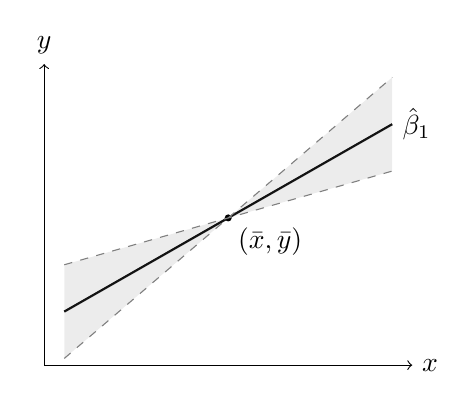
\begin{tikzpicture}[scale=0.85]
				\draw[->] (0,0) -- (5.5,0) node[right] {$x$};
				\draw[->] (0,0) -- (0,4.5) node[above] {$y$};
				\coordinate (P) at (2.75,2.2);
				\fill (P) circle (1.5pt) node[below right] {$(\bar x,\bar y)$};
				\draw[thick] (0.3,0.8) -- (5.2,3.6) node[right] {$\hat\beta_1$};
				\draw[dashed,gray] (0.3,1.5) -- (5.2,2.9);
				\draw[dashed,gray] (0.3,0.1) -- (5.2,4.3);
				\fill[gray,opacity=0.15] (0.3,0.1) -- (5.2,4.3) -- (5.2,2.9) -- (0.3,1.5) -- cycle;
			\end{tikzpicture}
		\end{column}
	\end{columns}
\end{frame}


\section{Partitioning Variability: The ANOVA Identity}


\begin{frame}{Splitting Total Variation}
	\[
		\underbrace{\sum_i(y_i-\bar y)^2}_{SST} \;=\; \underbrace{\sum_i(\hat y_i-\bar y)^2}_{SSR} \;+\; \underbrace{\sum_i(y_i-\hat y_i)^2}_{SSE}
	\]

	\begin{itemize}
		\item $SST$: total variability in the response
		\item $SSR$: variability \emph{explained} by the regression on $x$
		\item $SSE$: variability left \emph{unexplained} (residual)
	\end{itemize}
\end{frame}


\begin{frame}{Degrees of Freedom Split the Same Way}
	\[
		\underbrace{n-1}_{SST} \;=\; \underbrace{1}_{SSR} \;+\; \underbrace{n-2}_{SSE}
	\]

	\begin{itemize}
		\item One degree of freedom for the regression --- a single slope parameter
		\item $n-2$ left for error, matching what was used for $MSE$
	\end{itemize}
\end{frame}


\begin{frame}{The ANOVA Table}
	\begin{table}
		\small
		\centering
		\begin{tabular}{lcccc}
			\toprule
			Source & df & SS & MS & $F_0$\\
			\midrule
			Regression & $1$ & $SSR$ & $MSR=SSR/1$ & $MSR/MSE$\\
			Residual (Error) & $n-2$ & $SSE$ & $MSE=SSE/(n-2)$ & \\
			\midrule
			Total & $n-1$ & $SST$ & & \\
			\bottomrule
		\end{tabular}
	\end{table}
	\begin{itemize}
		\item Rows sum: the $df$'s add to $n-1$, the $SS$'s add to $SST$
	\end{itemize}
\end{frame}


\begin{frame}{ANOVA Table for the Example}
	\begin{table}
	\small
	\centering
	\begin{tabular}{lcccc}
		\toprule
		Source & df & SS & MS & $F_0$\\
		\midrule
		Regression & $1$ & $450$ & $450.0$ & $162.0$\\
		Residual & $18$ & $50$ & $2.778$ & \\
		\midrule
		Total & $19$ & $500$ & & \\
		\bottomrule
		\end{tabular}
	\end{table}
	\begin{itemize}
		\item $SSR=\hat\beta_1 S_{xy}=1.5(300)=450$
		\item $F_0 = 450/2.778 = 162.0$
	\end{itemize}
\end{frame}


\section{The F-Test for Significance of Regression}


\begin{frame}{$F$-Test}
	\[
		F_0 = \frac{MSR}{MSE} \sim F_{1,\,n-2} \quad\text{under } H_0:\beta_1=0
	\]
	\begin{itemize}
	\item Reject $H_0$ if $F_0 > F_{\alpha,\,1,\,n-2}$
	\item For the example: $F_{0.05,1,18}=4.41$; since $F_0=162.0 \gg 4.41$, reject $H_0$
	\end{itemize}
\end{frame}


\begin{frame}{$F$-Test vs.\ $t$-Test: Same Question, Two Routes}
	\begin{itemize}
	\item[] \textbf{Question:} in simple linear regression, how do the $t$-test and $F$-test for $H_0:\beta_1=0$ relate?
	% Answer: they are algebraically equivalent. F_0 = t_0^2, and the critical
	% values match too: F_{alpha,1,n-2} = t_{alpha/2,n-2}^2. In SLR the F-test
	% gives no new information beyond the two-sided t-test on beta_1.
	\end{itemize}

	\svspace{1em}

	\begin{itemize}
		\item Check against the numbers above: $t_0^2=12.72^2=161.8\approx F_0=162.0$ (rounding)
		\item In \emph{multiple} regression the $F$-test generalizes to several predictors at once; the simple $t$-test does not
	\end{itemize}
\end{frame}


\section{Coefficient of Determination}


\begin{frame}{$R^2$: How Much Variation Is Explained}
	\[
		R^2 = \frac{SSR}{SST} = 1-\frac{SSE}{SST}, \qquad 0\le R^2\le 1
	\]
	\begin{itemize}
		\item Proportion of the total variability in $y$ explained by the regression on $x$
		\item For the example: $R^2=450/500=0.90$ --- 90\% of the variability in sales is explained by advertising expenditure
	\end{itemize}
\end{frame}


\begin{frame}{$R^2$ and the Correlation Coefficient}
	\begin{itemize}
		\item In simple linear regression only:
	\end{itemize}
	\[
		R^2 = r^2
	\]
	\begin{itemize}
		\item $r=\sqrt{R^2}=\sqrt{0.90}=0.949$ (sign taken from $\hat\beta_1$)
		\item This equivalence is special to SLR --- it does \emph{not} hold once there is more than one predictor
	\end{itemize}
\end{frame}


\section{Prediction}


\begin{frame}{Two Different Questions}
	\begin{itemize}
		\item Fix a value $x_0$. Two distinct targets:
		\begin{itemize}
			\item the \emph{mean} response $E[Y\mid x_0]=\beta_0+\beta_1 x_0$
			\item a \emph{single new} observation $Y_0=\beta_0+\beta_1 x_0+\varepsilon_0$
		\end{itemize}
		\item Both are estimated by the same point, $\hat y_0=\hat\beta_0+\hat\beta_1 x_0$
		\item But they do \emph{not} share the same uncertainty
	\end{itemize}
\end{frame}


\begin{frame}{Confidence Interval for the Mean Response}
	\[
		\Var(\hat y_0) = \sigma^2\left(\frac1n+\frac{(x_0-\bar x)^2}{S_{xx}}\right)
	\]
	\[
		\hat y_0 \pm t_{\alpha/2,\,n-2}\sqrt{MSE\left(\frac1n+\frac{(x_0-\bar x)^2}{S_{xx}}\right)}
	\]
	\begin{itemize}
		\item Narrowest at $x_0=\bar x$, widening as $x_0$ moves away from $\bar x$
	\end{itemize}
\end{frame}


\begin{frame}{Prediction Interval for a New Observation}
	\[
		\Var(Y_0-\hat y_0) = \sigma^2\left(1+\frac1n+\frac{(x_0-\bar x)^2}{S_{xx}}\right)
	\]
	\[
		\hat y_0 \pm t_{\alpha/2,\,n-2}\sqrt{MSE\left(1+\frac1n+\frac{(x_0-\bar x)^2}{S_{xx}}\right)}
	\]
	\begin{itemize}
		\item The extra ``$1$'' accounts for the variability of $\varepsilon_0$ itself, on top of the uncertainty in estimating the line
		\item Always wider than the CI for the mean response
	\end{itemize}
\end{frame}


\begin{frame}{CI and PI at $x_0=12$: The Example}
	\begin{align*}
		\hat y_0 &= 35+1.5(12) = 53\\
		se(\text{mean}) &= \sqrt{2.778\left(\tfrac{1}{20}+\tfrac{4}{200}\right)} = 0.441\\
		se(\text{pred}) &= \sqrt{2.778\left(1+\tfrac{1}{20}+\tfrac{4}{200}\right)} = 1.724
	\end{align*}
	\begin{itemize}
		\item 95\% CI for the mean response: $53\pm 2.101(0.441)=(52.1,\ 53.9)$
		\item 95\% PI for a new observation: $53\pm 2.101(1.724)=(49.4,\ 56.6)$
	\end{itemize}
\end{frame}


\begin{frame}{CI Band vs.\ PI Band}
	\begin{columns}[T]
		\begin{column}{0.45\textwidth}
			\begin{itemize}
				\item Both bands are narrowest at $x=\bar x$ and flare outward
				\item The PI band is always the wider of the two, everywhere
				\item Neither band should be trusted far outside the range of the observed $x_i$
			\end{itemize}
		\end{column}
		\begin{column}{0.55\textwidth}
			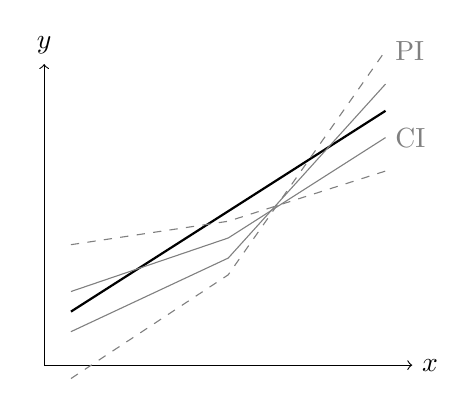
\begin{tikzpicture}[scale=0.85]
				\draw[->] (0,0) -- (5.5,0) node[right] {$x$};
				\draw[->] (0,0) -- (0,4.5) node[above] {$y$};
				\draw[thick] (0.4,0.8) -- (5.1,3.8);
				\draw[gray] (0.4,1.1) -- (2.75,1.9) -- (5.1,3.4);
				\draw[gray] (0.4,0.5) -- (2.75,1.6) -- (5.1,4.2);
				\draw[gray,dashed] (0.4,1.8) -- (2.75,2.15) -- (5.1,2.9);
				\draw[gray,dashed] (0.4,-0.2) -- (2.75,1.35) -- (5.1,4.7);
				\node[gray,right] at (5.1,3.4) {CI};
				\node[gray,right] at (5.1,4.7) {PI};
			\end{tikzpicture}
		\end{column}
	\end{columns}
\end{frame}


\begin{frame}{Extrapolation Warning}
	\begin{itemize}
		\item Both intervals are derived under the model fit \emph{within} the observed range of $x$
		\item Predicting far outside that range assumes the linear relationship continues to hold --- often unjustified
		\item[] \textbf{Question:} in the advertising example ($x$ ranging roughly 5--15), how much would you trust a prediction at $x_0=40$?
		% Answer: very little -- x0=40 is far outside the observed range, so the
		% formula still produces a number but the linear-model assumption backing
		% it has never been checked out there. Treat it as extrapolation, not
	% interpolation.
	\end{itemize}
\end{frame}


\section{Summary}


\begin{frame}{Putting It Together}
	\begin{itemize}
		\item $\hat\beta_0,\hat\beta_1$ are normal; standardized by their standard errors they become $t_{n-2}$
		\item $t$-tests and CIs for $\beta_0,\beta_1$ follow the same template throughout
		\item ANOVA partitions $SST=SSR+SSE$; the $F$-test for $\beta_1=0$ is equivalent to the $t$-test in SLR
		\item $R^2=SSR/SST=r^2$ measures explained variability, not model correctness
		\item Mean-response CIs are narrower than new-observation PIs --- know which one you need
	\end{itemize}
	\svspace{0.5em}
	\begin{itemize}
		\item[] \textbf{Next time:} multiple linear regression
	\end{itemize}
\end{frame}